\documentclass{beamer}
\usepackage{listings}
\usepackage{xcolor}
\usepackage{hyperref}
\usepackage{graphicx}
%\usepackage[utf8]{inputenc}
\usefonttheme[onlymath]{serif}
%\usepackage[T1]{fontenc}

\usepackage{xeCJK}
\setCJKmainfont{Noto Sans CJK SC}
\setCJKsansfont{Noto Sans CJK SC}
\setCJKmonofont{Noto Sans CJK SC}

\usetheme{Madrid}
\definecolor{codegreen}{rgb}{0,0.6,0}
\definecolor{codegray}{rgb}{0.5,0.5,0.5}
\definecolor{codepurple}{rgb}{0.58,0,0.82}
\definecolor{backcolour}{rgb}{0.95,0.95,0.92}
\lstdefinestyle{mystyle}{
    backgroundcolor=\color{backcolour},   
    commentstyle=\color{codegreen},
    keywordstyle=\color{magenta},
    numberstyle=\tiny\color{codegray},
    stringstyle=\color{codepurple},
    basicstyle=\ttfamily\footnotesize,
    breakatwhitespace=false,         
    breaklines=true,                 
    captionpos=b,                    
    keepspaces=true,                 
    numbers=left,                    
    numbersep=5pt,                  
    showspaces=false,                
    showstringspaces=false,
    showtabs=false,                  
    tabsize=2
}
\lstset{style=mystyle}

\usepackage{xparse}

\title{Tweets Sentiment Analysis}
\author{Kuo-Wei Ho\inst{1}, Hao-Chien Wang\inst{2}}

\institute[NTU]
{
	\inst{1}
	NTUEE
	\and
	\inst{2}
	NTUPhys
}
\date[DSP 2019]
{Data Science Programing, July 2019\\{\scriptsize Instructor: 蔡芸琤}\\{\scriptsize TA: 王冠人, 萬俊彥, 何承諭}}

\begin{document}

\frame{\titlepage}

\begin{frame}{Table of Contents}
	\tableofcontents
\end{frame}


\section{Problem}%
\label{sec:problem}

\begin{frame}{Problem}
	Given a set of data containing 1,600,000 tweets and the sentiment of each tweets. Create a model that can analyze sentiment of new tweets.\\
	\begin{table}[htpb]
		\tiny
		\centering
		\caption{Data example}
		\label{tab:data}
		\begin{tabular}{c c c c}
			sentiment & Post ID & User ID & tweets \\
			\hline
			 0 & 1467814192 & Ljelli3166 & blagh class at 8 tomorrow  \\
			 0 & 1467821455 & CiaraRenee & I need a hug  \\
			 4 & 1677796507 & FoodAllergyBuzz & @otibml Thx for the tweet!  \\
			 4 & 1677796519 & Iakido & Sunshine.....I LOVE this weather!!!  \\
		\end{tabular}
	\end{table}
	0: Negative \\
	4: Positive \\
	{\scriptsize Data: \url{https://www.kaggle.com/kazanova/sentiment140}} \\
	{\scriptsize Github link: \url{https://github.com/b07901135/2019dsp-summer-project}}
\end{frame}


\section{Key tools}%
\label{sec:key_tools}



\begin{frame}{Key Tools}
	\begin{itemize}
		\item Vectorizing text: \textit{GloVe (Global Vectors for Word Representation} by Standford University.)
		\item Neural network: \textit{RNN (Recurrent Neural Network)}
	\end{itemize}
\end{frame}

\section{Steps}%
\label{sec:steps}

\begin{frame}{Steps: Overview}
	\begin{enumerate}
		\item Clean the data: remove non-UTF8 symbols, numbers and URLs.
		\item Combine all tweets into one string and tokenize.
		\item Feed the tokens to GloVe to generate word vectors.
		\item Tokenize all tweets and search each words in the vectors to transform it into a list of matrices.
		\item Train the RNN model with the list of metrices.
	\end{enumerate}	
\end{frame}

\begin{frame}{Steps: Overview}
    \begin{figure}[h]
        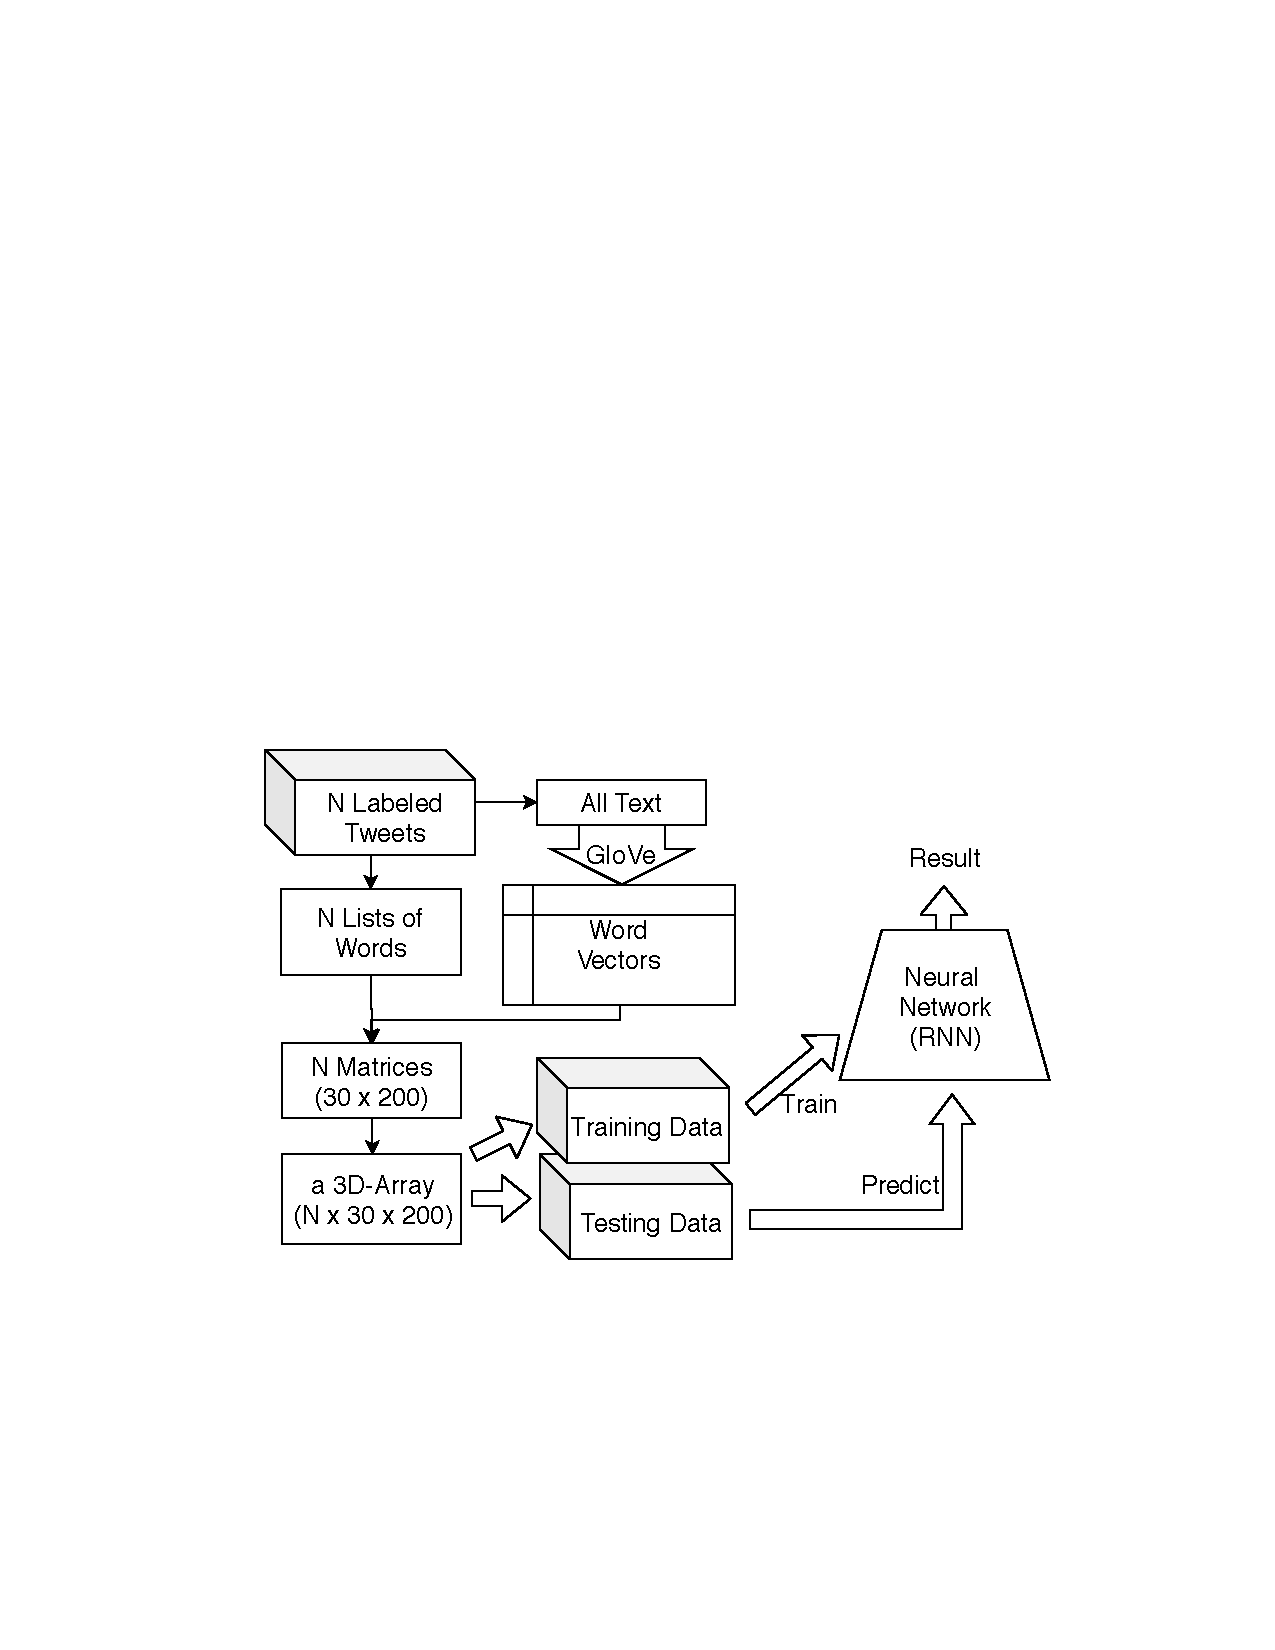
\includegraphics[trim={2cm 5cm 0 12cm},clip,height=3in]{img/flow_chart.pdf}
        \label{fig:}
    \end{figure}
\end{frame}

\begin{frame}{Steps: Data Cleaning and Vectorization}
	\begin{enumerate}
		\item Replace URLs as ``url''
		\item Replace name tags ( e.g. @allen1234 ) as ``names''
		\item Remove other non-UTF8 characters (\textit{stri\_enc\_toutf8()} doesn't help)
		\item Combine tweets into a string, tokenize and remove stopwords.
		\item Generate TCM, feed it to the neural network to fit the model.
		\item Generate word vectors ( $Dim = 200 $ ).
	\begin{table}[htpb]
		\scriptsize
		\centering
		\caption{Word vectors}
		\label{tab:wordVec}
		\begin{tabular}{c | c c c c c}
			"peanuts" & -0.55638 & 0.04843 & -0.14483 & -0.47563 & \ldots \\
			"permission" & 0.15835 & 0.06962 & 0.04398 & -0.27275 & \ldots \\ 
			"beast" & -0.20607 & 0.16818 & -0.17708 & -0.26557 & \ldots \\
			"eva" & 0.32598 & 0.04554 & -0.72075 & -0.04571 & \ldots \\
			"pounding" & 0.67231 & 0.00862 & -0.07067 & -0.15407 & \ldots \\
		\end{tabular}
	\end{table}
	\end{enumerate}
\end{frame}

\begin{frame}{Steps: Tweets Vectorization}
	\begin{itemize}
		\item Discard data other than \textbf{sentiment} and \textbf{tweets text}
		\item Tokenize tweets and lookup the tokens in the word vectors.
		\item Discard tweets containing more than \textbf{30 tokens} so that the matrices will not contain too much zeros.
		\item \textbf{Due to the limitation of RAM size, we are only able to use 50,000 tweets data.} 

	\end{itemize}
	\begin{table}[htpb]
		\scriptsize
		\centering
		\caption{Data manipulation}
		\label{tab:dataMan}
		\begin{tabular}{c c}
			sentiment & tweets \\
			\hline
			 0 & blagh class at 8 tomorrow  \\
			 0 & I need a hug  \\
			 4 & @otibml Thx for the tweet!  \\
			 4 & Sunshine! I LOVE this weather!!!  \\
		\end{tabular}
		$\Rightarrow$
		\begin{tabular}{c c}
			sentiment & tweets \\
			\hline
			 0 & blagh class at num tomorrow \\
			 0 & I need a hug \\
			 4 & name Thx for the tweet\\
			 4 & Sunshine! I LOVE this weather!!! \\
		\end{tabular}
		$\Rightarrow$
		\begin{tabular}{c c}
			sentiment & tweets \\
			\hline
			0 & $ \mathbf{A}_{ 30 \times 200 }  $ \\
			0 & $ \mathbf{B}_{ 30 \times 200 }  $ \\
			4 & $ \mathbf{C}_{ 30 \times 200 }  $ \\
			4 & $ \mathbf{D}_{ 30 \times 200 }  $ \\
		\end{tabular}
	\end{table}
	
\end{frame}

\begin{frame}{Steps: RNN Fitting}

    \begin{figure}[h]
        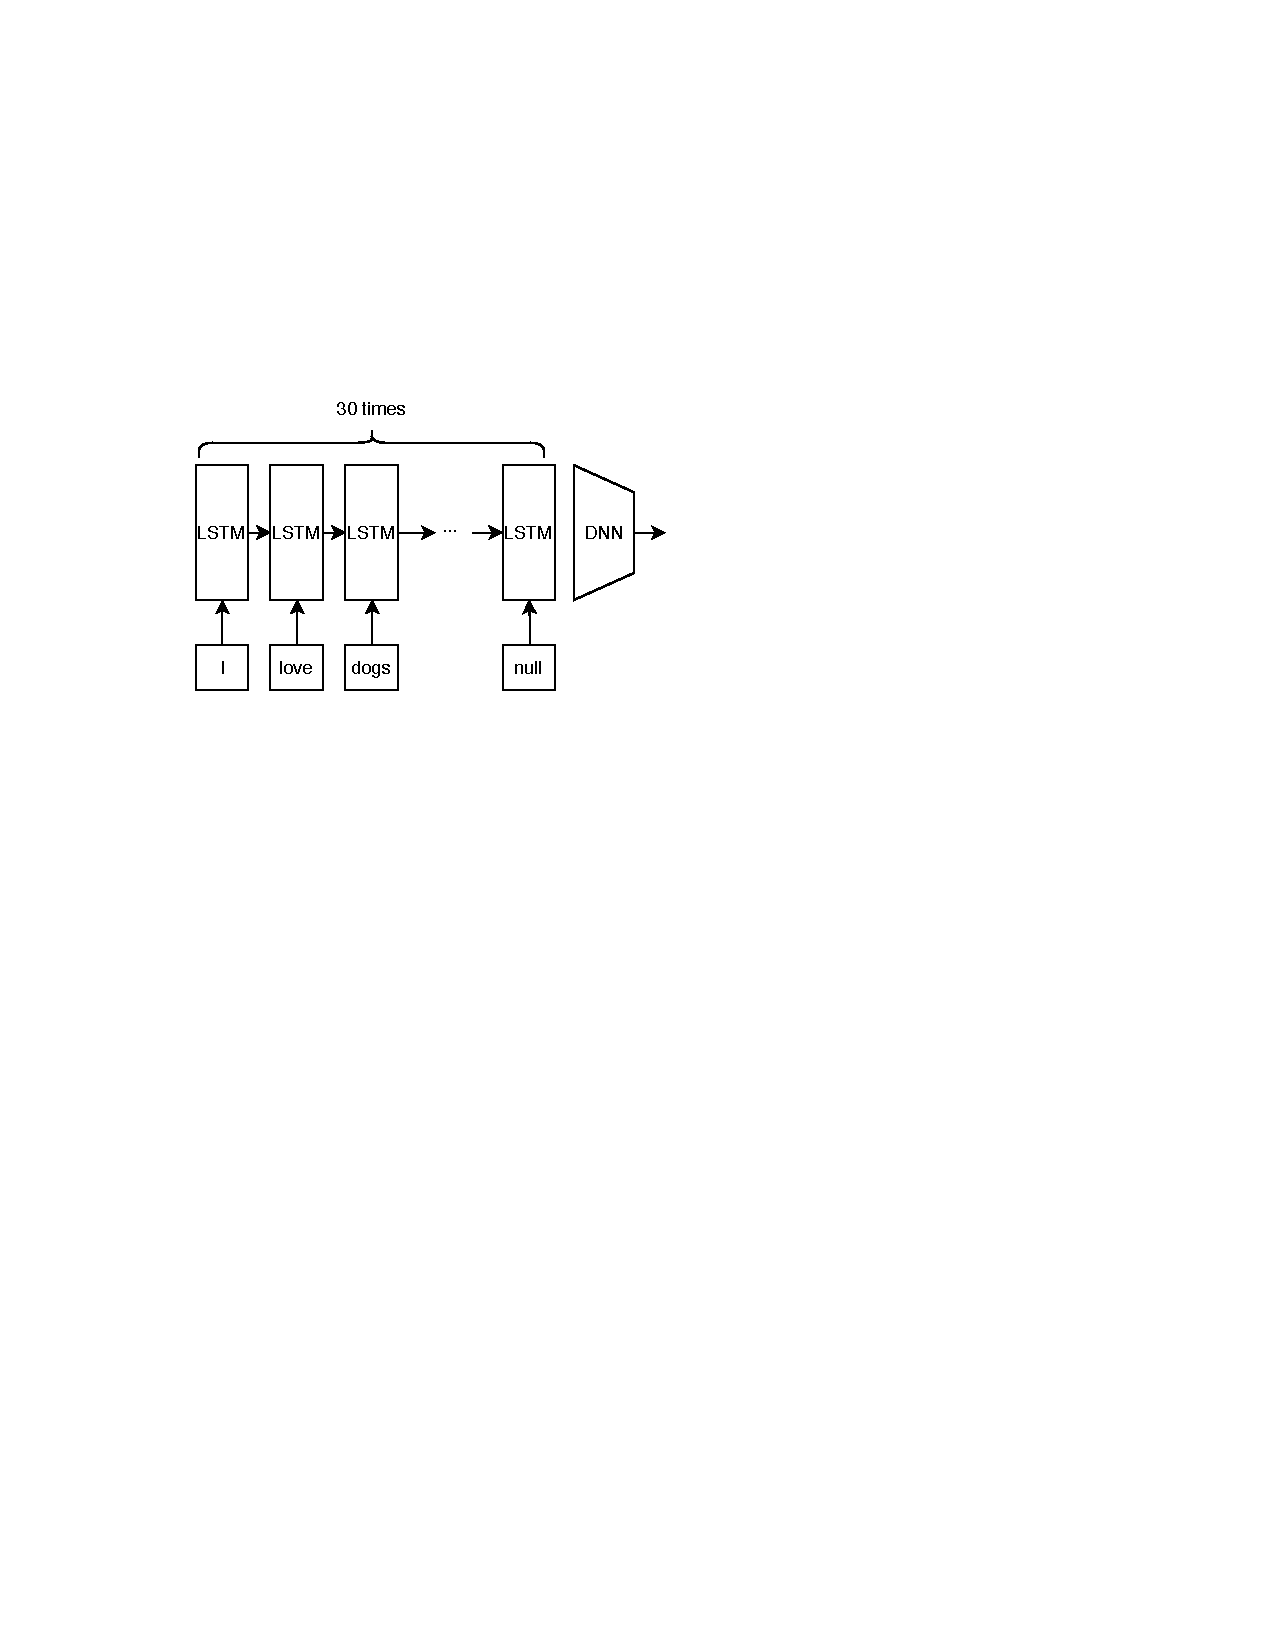
\includegraphics[trim={1cm 12cm 0 6cm},clip]{img/rnn.pdf}
    \end{figure}
		
\end{frame}

\section{Results}%
\label{sec:results}
\begin{frame}{Result}
    \begin{itemize}
        \item The best result we got is a precision of 78.68\% (5000 testing data).
    \end{itemize}
    \begin{figure}[h]
        \centering
        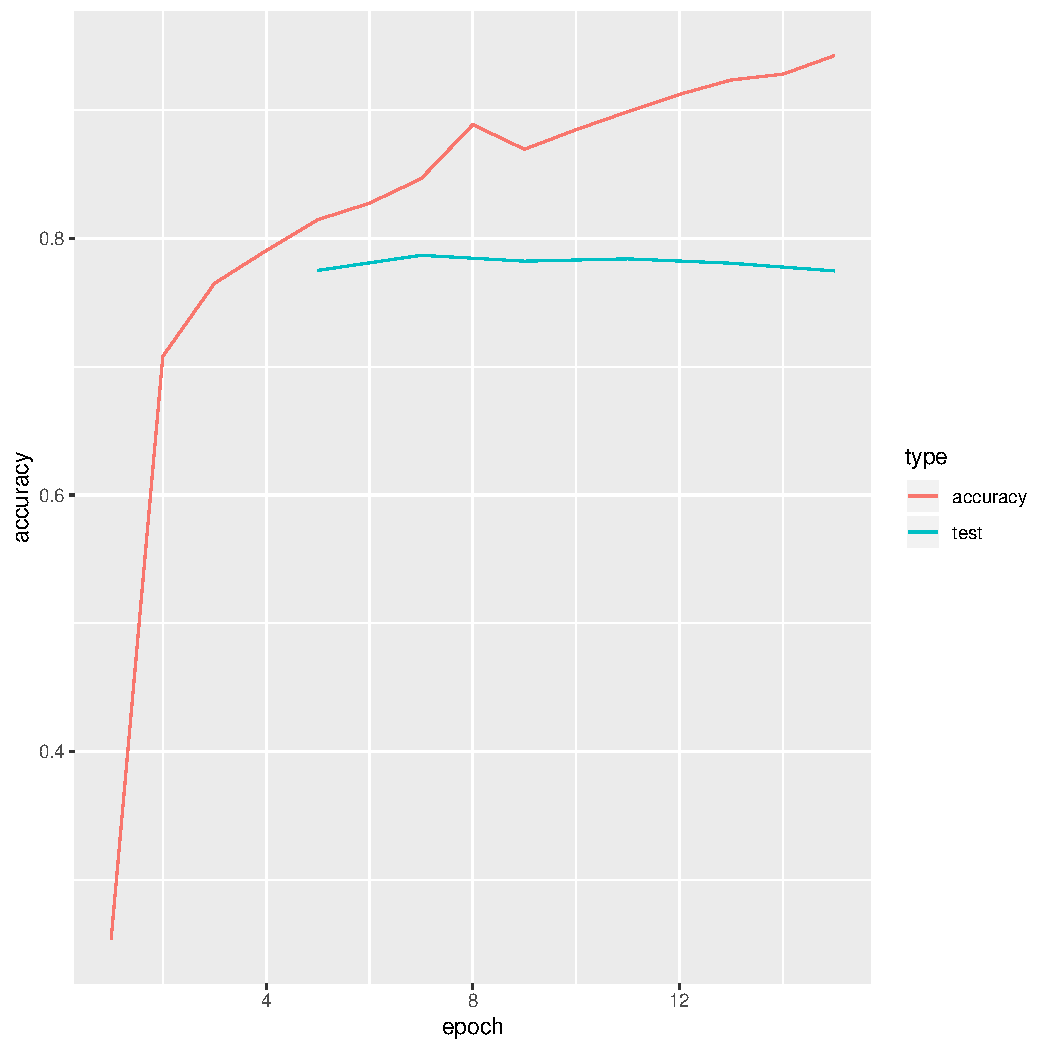
\includegraphics[width = 0.45 \textwidth]{../data_rnn/plot/accplot.pdf}
        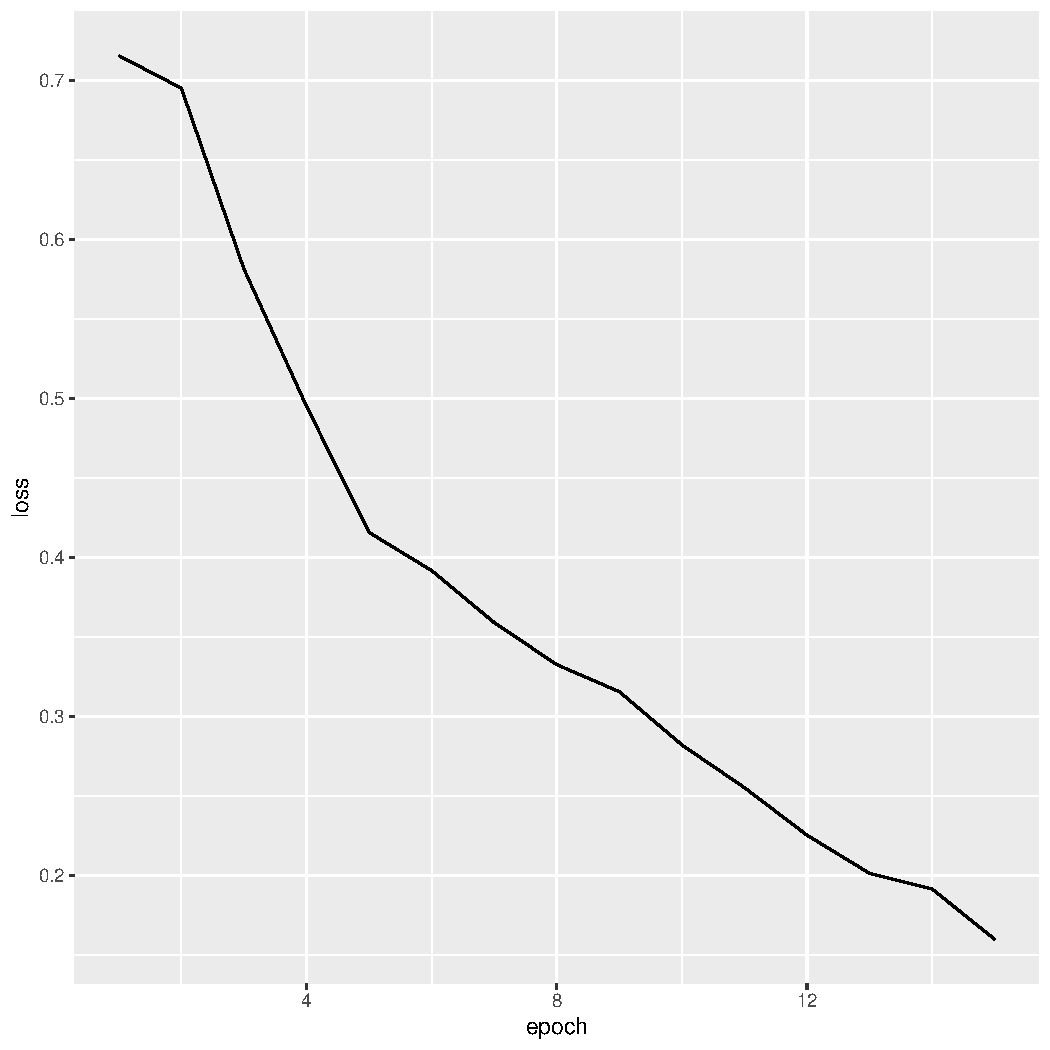
\includegraphics[width = 0.45 \textwidth]{../data_rnn/plot/lossplot.pdf}
        \caption{Training process.\label{fig:result}}
    \end{figure}

\end{frame}
\section{Difficulties encountered}%
\label{sec:difficulties_encountered}


\begin{frame}{Difficulties Encountered}
	\begin{enumerate}
		\item Hardware limitations (Ram size, CPU/GPU speed): Kill X session, \texttt{gc()/remove()}
		\item Package problems (Tensorflow)
		\item Carelessness on manipulating data, leading to incorrect results.
		\item Large data size causing difficulties checking results and big waste of time.
		

	\end{enumerate}
\end{frame}


\begin{frame}{Dark Magic}
	\begin{itemize}
		\item \texttt{save()/load()}
		\item \texttt{pbapply}
		\item \texttt{gc()}
		\item \texttt{rm()}
		\item \texttt{abind()}
		\item \texttt{melt()}

	\end{itemize}
	
\end{frame}


\end{document}


